\chapter{Channel Estimation}
\label{ch:ChEst}

LTE was chosen as the standard to use here as it is very mature and has readily available MATLAB/Labview based implementation. In the case of this thesis the aim is not to reinvent standard by redesigning pilot symbol placements. Instead existing standards were used in order to collect experimental data. This reduces design time and focusses more on the issue at hand which is channel estimation data of a MIMO Channel.

\section{OFDM}\label{sec:OFDM}
LTE is based on OFDMA in the physical layer which is a multi carrier communication scheme \cite{FazelKaiser}. As the name suggests OFDM uses orthogonal sub carriers from an orthonormal system to form the basis for independent data streams. For band limited transmission systems with finite access time per channel use the dimension of the parallel data stream is given by the equation \ref{eq:BandLim}  \cite{UtschickOFDM}.

        \begin{equation} \label{eq:BandLim}
            N = BT
        \end{equation}

        \begin{table}[H]
            \begin{center}
                \begin{tabular}{|c|l|}
                    \hline
                    Parameter& Description\\ \hline
                    $N$& Dimension of system \\ \hline
                    $B$& Signal Bandwidth \\ \hline
                    $T$& Channel access time \\
                    \hline
                \end{tabular}
                \caption{}
                \label{tab:BandLimTrans}
            \end{center}
        \end{table}

The orthonormal basis function can be mathematically modelled as the equation \ref{eq:OFDM} \cite{UtschickOFDM}.

        \begin{equation} \label{eq:OFDM}
            \begin{split}
                \psi_{b,q} = p_{T_{b}}(t)exp(j2{\pi}q{\frac{t}{T}}) \\
                p_{T_{b}}(t) = \left\{
                    \begin{matrix}
                        1; & t \in T_b \\
                        0; & otherwise \\
                    \end{matrix}\right.
            \end{split}
        \end{equation}

        \begin{table}[H]
            \begin{center}
                \begin{tabular}{|c|l|}
                    \hline
                    Parameter& Description\\ \hline
                    $\psi_{b,q}$& normalized orthogonal basis functions\\ \hline
                    $b$& channel access slot\\ \hline
                    $q$& sub carrier index\\ \hline
                    $T$& channel access time \\ \hline
                    $T_{b}$& $ bT \leq t < (b + 1)T \subset \mathbb{R}$ \\ \hline
                \end{tabular}
                \caption{}
                \label{tab:OFDMParam}
            \end{center}
        \end{table}


        The transmitted data can hence be modelled as the following
        \begin{equation} \label{eq:TxDataMath}
            x_b(t) = \sum_{q=0}^{N-1}\underbrace{X_{b,q}}_\text{data} \psi_{b,q}(t)
        \end{equation}

        For a given ideal AWGN Channel, where there is no delay spread or multipath propogation, the corresponding received data is modelled as
        \begin{equation} \label{eq:RxDataMathIdeal}
            y_b(t) = \sum_{q=0}^{N-1}x_b(t) \psi_{b,q}(t) +\eta_b(t)
        \end{equation}
        where $\eta_b(t)$ is the additive noise

        The demodulation is based on the same set of orthonormal basis vectors as that of the transmitter, hence we have
        \begin{equation}
            \begin{aligned}\label{eq:InnerProductRxIdeal}
                \hat{x}_{b,q} = \langle y,\psi_{b,q}(t)\rangle + \langle\eta_{b},\psi_{b,q}(t)\rangle = x_{b,q}(t) + \eta_{b,q} & & & \forall q = 1,...,N \\
            \end{aligned}
        \end{equation}

        In the case of a channel with a delay spread (also referred to as multipath propogations) we model it as the following
        \begin{equation} \label{eq:DelaySpread}
            \begin{split}
                h(t) = \sum_{l=0}^{L-1}h_l\delta{(t-l\frac{T}{N})} \\ 
            \end{split}
        \end{equation}
        this causes the term $h_lx_{b,q}\psi_q(t-l\frac{T}{N}-bT)$ which leads to interference between adjacent channels $T_{b-1},T_{b},T_{b+1}$, etc.

\subsection{Cyclic Prefix}\label{ssec:CP}

As a result of Equation \ref{eq:DelaySpread} we have to compensate for the interference of the symbols of the $b_{th}$ channel with the other channels. A simple solution to this interference is a Cyclic prefix. As the name suggests it is a cyclic addition of the signal at the transmitter end, which means copying the beginning of the signal and adding it to the end. To this end $T = T + T_p$, where $T_p$ is the duration of the cyclic prefix. In the LTE standard the durations are predefined based the normal or extended mode \cite{3gpp36211}

\begin{equation}
    \begin{split}
        \psi_{b,q}(t) = p_{T_b}(t)exp\left( j2\pi{q}\frac{t}{T} \right) \\
        \text{where} \; \psi_{b,q} \in T_b = [-T_p + bT_s , bT_s + T [
    \end{split}
\end{equation}

This is illustrated in the Figure \ref{fig:CPIlls}

\begin{figure}[H]
    \begin{center}
        \includegraphics[width=\linewidth]{images/CP_illustration.png}
        \caption{Cyclic prefix addition \cite{UtschickOFDM}}
        \label{fig:CPIlls}
    \end{center}
\end{figure}

On the receiver end

\begin{equation}
    y_{b,n} = \sum_{l=1}^{L-1}h_l\delta_{n-l} \ast \sum_{l=-Np}^{N-1}x_{b,k}\delta_{n-k} = \sum_{l=1}^{L-1}\sum_{k=-Np}^{N-1}h_lx_{b,k}\delta_{n-l-k}
\end{equation}

subject to $L-1 \leq N_p$ ,where $N_p$ is the number of samples of the cyclic prefix

\begin{equation}
    \begin{aligned}
        y_{b,n} & = \sum_{l=1}^{L-1}h_lx_{b,n-l} = \sum_{l=1}^{L-1}h_lx_{b,mod_N(n-l)}, & & n,q \in 0,\cdots ,N-1
        \\
        y_{b,n} & = h_n \circ x_{b,n} \Leftrightarrow \frac{1}{N}Y_{b,q} = H_qX_{b,q}, & & n,q \in 0,\cdots,N-1
    \end{aligned}
\end{equation}

\begin{equation}\label{eq:MatrixConvCP}
    \begin{bmatrix}
        y_{b,-2}
        \\ y_{b,-1}
        \\ y_{b,0}
        \\ y_{b,1}
        \\ y_{b,2}
        \\ y_{b,3}
    \end{bmatrix}
    =
    \begin{bmatrix}
        h_0 &  &  &  &  & \\ 
        h_1 & h_0 &  &  &  & \\ 
        h_2 & h_1 & h_0 &  &  & \\ 
        & h_2 & h_1 & h_0 &  &  \\ 
        & & h_2 & h_1 & h_0 &  \\ 
        & & & h_2 & h_1 & h_0
    \end{bmatrix}
    \begin{bmatrix}
        x_{b,-2}
        \\ x_{b,-1}
        \\ x_{b,0}
        \\ x_{b,1}
        \\ x_{b,2}
        \\ x_{b,3}
    \end{bmatrix}
    +
    \begin{bmatrix}
        h_2 & h_1 & & & & \\ 
        &  h_2 &  &  &  & \\ 
        &  &  &  &  & \\ 
        &  &  &  &  & \\ 
        &  &  &  &  & \\ 
        &  &  &  &  & 
    \end{bmatrix}
    \begin{bmatrix}
        x_{b-1,2} \\ 
        x_{b-1,3} \\ 
        0 \\
        0 \\ 
        0 \\ 
        0 
    \end{bmatrix}
    +
    \begin{bmatrix}
        \eta_{b,-2}\\ 
        \eta_{b,-1}\\ 
        \eta_{b,0}\\ 
        \eta_{b,1}\\ 
        \eta_{b,2}\\ 
        \eta_{b,3}
    \end{bmatrix}
\end{equation}

With a cyclic prefix chosen such that $x_{b,-n} = x_{b,N-n}, n \leq N_p $, then $x_{b,-1}$ and $x_{b,-2}$ can be deleted and equation \ref{eq:MatrixConvCP} can be rearranged as the following

\begin{equation}\label{eq:MatrixConvCPSimpl}
    \begin{bmatrix}
        y_{b,0}
        \\ y_{b,1}
        \\ y_{b,2}
        \\ y_{b,3}
    \end{bmatrix}
    = 
    \begin{bmatrix}
        h_0 &  &h_2 & h_1 \\ 
        h_1 & h_0 & & h_2 \\ 
        h_2 & h_1 & h_0 & \\ 
        & h_2 & h_1 & h_0
    \end{bmatrix}
    \begin{bmatrix}
        x_{b,0}
        \\ x_{b,1}
        \\ x_{b,2}
        \\ x_{b,3}
    \end{bmatrix}
    +
    \begin{bmatrix}
        \eta_{b,0}\\ 
        \eta_{b,1}\\ 
        \eta_{b,2}\\ 
        \eta_{b,3}
    \end{bmatrix}
\end{equation}

Taking the DFT of equation \ref{eq:MatrixConvCPSimpl} gives 

\begin{equation}\label{eq:DFTCP}
    y_b = \hat{H}x_b + \eta_{b} \Leftrightarrow Y_b = \frac{1}{N}F\hat{H}F^HX_b + F\eta_{b}
\end{equation}

Where $F$ is the fourier matrix. Since $\hat{H}$ is a circulant matrix (also a convolutional matrix) it can be broken down as equation \ref{eq:CircMtxExp} \cite{CircMatrixStanford}. The eigenvalues of the circulant matrix are the fourier transformed coefficients of the first column while the eigenvectors are the columns of the inverse fourier transform matrix. Equation \ref{eq:CircMtxExp} presents a eigenvector decomposition of matrix $H$ where $F^H$ is the inverse DFT matrix and $\Lambda$ is the diagonal matrix with entries being the fourier transform terms of the first column of the matrix $H$.

\begin{equation}\label{eq:CircMtxExp}
    \begin{aligned}
        \hat{H} & = U\Lambda U^{-1}  & = \frac{1}{N}F^H \Lambda F\\
          \frac{1}{N}F\hat{H}F^H    & = \Lambda
    \end{aligned}
\end{equation}

Therefore equation \ref{eq:DFTCP} simplifies to 

\begin{equation}\label{eq:OFDMFinalEq}
    \begin{aligned}
        Y_b & = \Lambda{X_b} + F\eta_b \\ & \text{or} \\
        Y_b & = diag({X_b}){H} + F\eta_b
    \end{aligned}
\end{equation}

where $\Lambda$, is a diagonal matrix and ${H}$ is the vector of channel coefficients in the frequency domain and decouples the subcarrier distortions with each other. Because of the cyclic prefix converting linear convolution into cyclic convolution, the received signal in the frequency domain is linearly dependent \textbf{only} on the corresponding frequency component of the channel propogation effect.


\subsection{Pilot assisted channel estimation}\label{ssec:PilotAssistedChEst}

%$\Lambda$ is therefore found easily which provides the channel coefficients in the frequency domain.

In order to determine the channel propogation effects known pilot symbols are inserted in the transmit frames as mentioned in section \ref{sssec:CRS} and the channel effects are inferred from the demodulated symbol on the receiver side. Although populating all the subcarriers with pilots is the best approach, this leads to high channel reference signal overheads and less data bandwidth. Hence in practical system implementations the only $P$ out of $N$ subcarriers carry the pilots and the rest are interpolated.

\begin{equation}\label{eq:OFDMChEstEq}
    \begin{aligned}
        Y & = XS{H} + \eta \\
    \end{aligned}
\end{equation}
$
Y \in \mathbb{C}^{P}, H \in \mathbb{C}^{N}, \eta \in \mathbb{C}^{P} \text{ are vectors}
\\ X = diag[X_{1},...,X_{P}] \in \mathbb{C}^{PxP}
\\ \text{and } S: \mathbb{C}^{N} \rightarrow \mathbb{C}^{P} \Rightarrow  H \mapsto H_P = [H_{s1},...,H{sp}]^T.
$
where $S$ is the selector matrix which selects $P$ out of $N$ subcarriers which carry the pilot symbols.

For non fully loaded OFDM systems which is typical in the real world the equation \ref{eq:OFDMChEstEq} reduces to the equation below.

\begin{equation}\label{eq:ReducedRankOFDMChEstEq}
    \begin{aligned}
        Y_P & = XH_P + \eta \\
    \end{aligned}
\end{equation}

{where } $H_P = SH$. A least squares estimate of the $H_P$ gives 

\begin{equation}\label{eq:ReducedRankOFDMChEstEq}
    \begin{aligned}
        \hat{H_{P,LS}} & = X^{-1}Y_P \\
    \end{aligned}
\end{equation}

$H_P$ is then subsequently interpolated across all the $N$ subcarriers. This can be done in many ways using either
\begin{itemize}
    \item Linear interpolation
    \item Sinc interpolation
    \item Cubic/Spline interpolation
    \item Wiener filters
\end{itemize}

\section{MIMO Channel Estimation}\label{sec:MIMO}

For the MIMO channel estimate the basics is the same as described in the section \ref{ssec:PilotAssistedChEst}, except in a $N_t{\times}N_r$ system we have $N_tN_r$ possible channels per subcarrier. This is explained as follows, from figure \ref{fig:MIMOChannel} it can be seen that there are $N_tN_r$ channels per subcarrier in the frequency domain. Equation \ref{eq:OFDMChEstEq} is used to calculate each channel. This is enabled by non interfering pilots for different antennas. This \textbf{must} be followed for faithful channel estimation and is a necissary criteria which has been followed in the LTE standard.

\begin{figure}[H]
    \begin{center}
        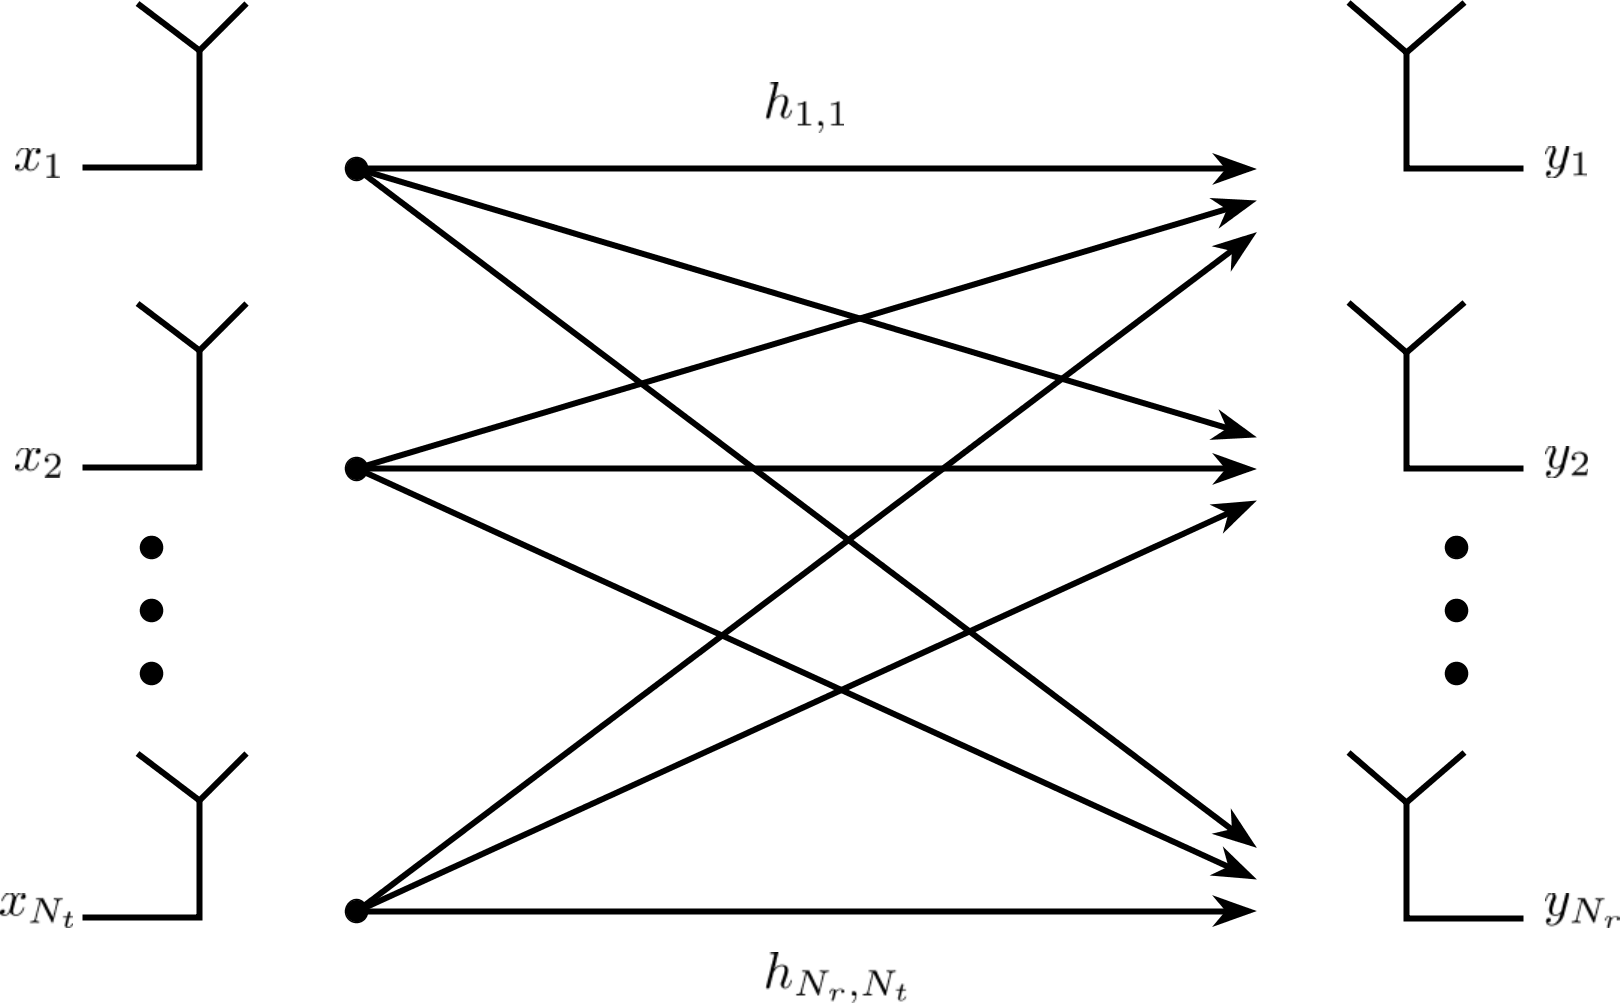
\includegraphics[width=\linewidth]{images/MIMO_Illustration.jpg}
        \caption{MIMO channel model}
        \label{fig:MIMOChannel}
    \end{center}
\end{figure}

\begin{equation}
    \hat{x} = Wy
\end{equation}

Once the channels propogation effects have been calculated each symbol has to be equalized to compensate the distortion effect caused by the dispersive channel. In the case of a MIMO channel there are 3 main algorithms which are

\subsection{Maximum Ratio Combiner}\label{ssec:Simple}

\begin{equation}
    W_{MRC} = C\hat{H}^H
\end{equation}
where $C$ is a diagonal matrix with 
$
C_{k,k} = \left ( \sum_{m}\left | H_{m,k} \right |^2 \right )^{-1}
$
and can be considered as a normaliser for the columns of the matrix $H$.

\subsection{Zero Forcing}\label{ssec:ZF}


\begin{equation}
    W_{ZF} = (\hat{H}^H\hat{H})^{-1}\hat{H}^H
\end{equation}

Zero forcing is an algorithm that is avoided although given its simplicity, the reason being that the noise can be amplified in the case of a low SNR situation. Hence in practice this algoritm is avoided. The implimentation is a Least squares estimate of the vector $\hat{x}$

\subsection{MMSE}\label{ssec:MMSE}

\begin{equation}
    W_{MMSE} = (\hat{H}^H\hat{H}+\sigma^{2}I)^{-1}\hat{H}^H
\end{equation}

where $\sigma$ is the inverse SNR.

MMSE algorithm performs the best under all situations. For high SNR scenarios it converges to an ZF algorithm and for a low SNR situation it converges to the MRC algorithm.
